\chapter{Envisioned Approach}
\begin{figure}
  \centering
  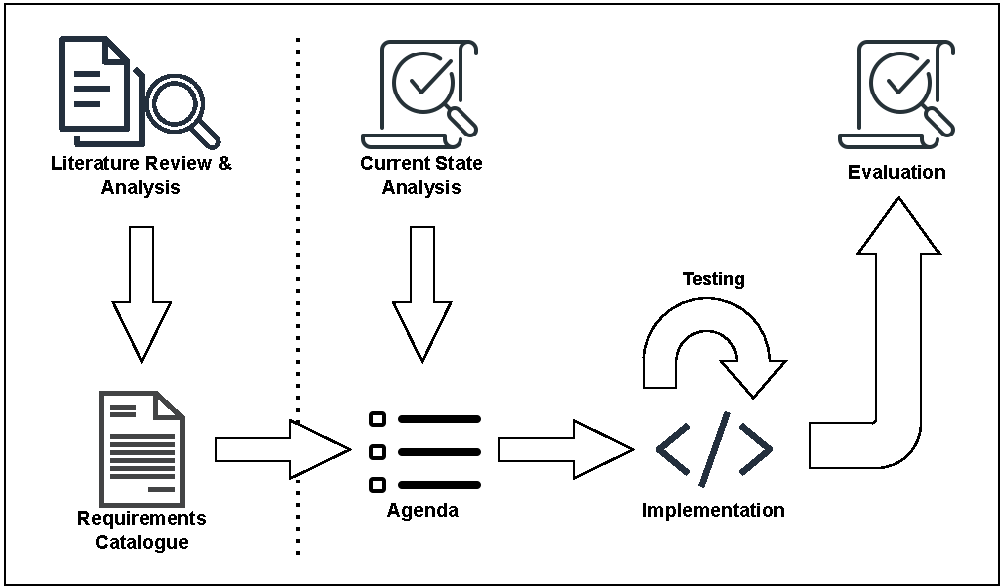
\includegraphics[width=0.75\textwidth]{img/approach_figure.pdf}
  \caption{Approach of the Thesis}
  \label{fig:approach_figure}
\end{figure}
Figure \ref{fig:approach_figure} visualises the general approach of the thesis showing distinct steps to meet the goal of the thesis.
The following sections describe each steps in more detail.

\section{Literature Review \& Analyzation}\label{approach:literature-review}
The edge computing simulation landscrape is vast with different simulators, which can have all different bias, metrics, implementations, characteristics and features.
For advancing ecoscape as a proper edge computing simulator, it is necessary to learn more about existing simulators and review as well as analyze their respective structure.

This step includes, defining which simulator is deemed to be part of the state of art and why, as well as analyze their respective metrics and their definitions as well as features and characteristics.

\section{Catalogue of Requirements}\label{approach:catalogue}
The reviews from section \ref{approach:literature-review} will be compared and evaluated to determine, what exactly is the state of art for simulators.
This results in the analysis of similarities and differences as well as their configurations to determine the requirements a simulator should meet.

\section{Ecoscape}\label{approach:ecoscape}
\subsection{Analyzation of Current State}\label{approach:ecoscape-current}
Firstly, to advance ecoscape in any way, the current state needs to be analyzed and compared to the catalogue to have a basic understanding how ecoscape can improve.

\subsection{Implementation}\label{approach:ecoscape-impl}
This step depends on the result of section \ref{approach:ecoscape-current} and is about implementing the missing features as well as improving existing features to meet the requirements of section \ref{approach:catalogue}'s catalogue.
The implementation will be done part of the ecoscape project and should be documented as well as steadily tested to guarantee satifying results.

\subsection{Evaluation}\label{approach:ecoscape-eval}
At the end, an evaluation takes place to determine if the resulting version of ecoscape is meeting expectations. This will be done via user study or expert interviews.
The exact parameters of said evaluation still need to be defined.

